\question{Электростатика триода. Распределение потенциала в плоском триоде}

Для того, чтобы найти распределение потенциала в плоском триоде, найдем
распределение потенциала в системе \( W_1 \), показанной на рисунке~\pic{20W1}.

\begin{figure}[h!]
  \center
  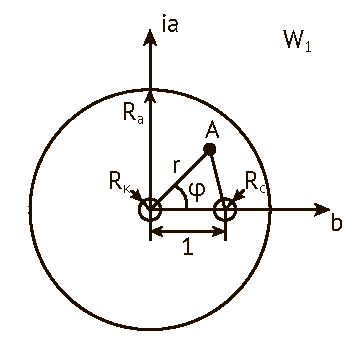
\includegraphics[width=.3\textwidth]{20_W1} \hspace{1em}
  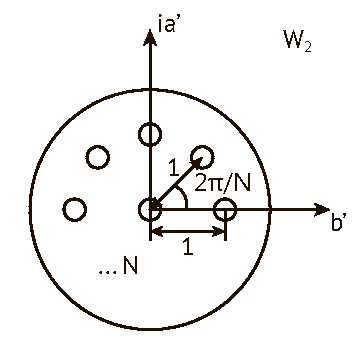
\includegraphics[width=.3\textwidth]{20_W2} \hspace{1em}
  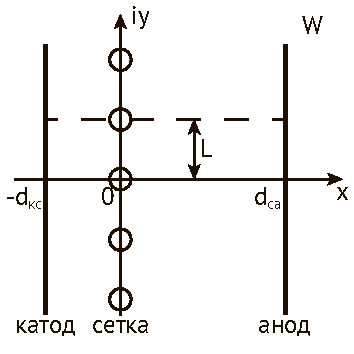
\includegraphics[width=.3\textwidth]{20_W} \\
  \parbox{.3\textwidth}{\caption{Комплексная плоскость \( W_1 \)}
    \label{pic20W1}} \hspace{1em}
  \parbox{.3\textwidth}{\caption{Комплексная плоскость \( W_2 \)}
    \label{pic20W2}} \hspace{1em}
  \parbox{.3\textwidth}{\caption{Комплексная плоскость \( W \)}
    \label{pic20W}}
\end{figure}

\( W_1 \) состоит из трех цилиндрических электродов: катода, несущего заряд
\( q_k \) и радиусом \( R_k \), элемента сетки, несущего \( q_c \) и радиусом
\( q_c \), и анода, радиусом \( R_a \). Между сеткой и катодом расстояние
принято за единицу. Радиусы сетки и катода значительно меньше расстояний между
сеткой и катодом и сеткой и анодом, поэтому их можно принять за точечные
заряженные стержни.

В точке \( A \) наводится следующий потенциал:
\begin{equation}
  U(r, \phi) = \frac{1}{2\pi\Ez}\left[ q_k\ln r + q_c\ln\sqrt{r^2 + 1 -
    2r\cos\phi} \right] + B.
  \label{eq20U1}
\end{equation}

Преобразуем комплексную плоскость по закону
\( W_2 = (W_1)^{1 / N} = (re^{i\phi})^{1 / N} \), где \( N \)~-- некоторое
число; получим систему \( W_2 \), изображенную на рисунке~\pic{20W2}.

Вместо одного элемента сетки в преобразованной системе будет \( N \) элементов,
отстоящих друг от друга на угол \( 2\pi / N \) и удаленных от катода на
расстояние, равном единице.

Преобразуем комплексную плоскость \( W_2 \) по закону
\[
  W = \ln(W_2) = \ln\left[ (re^{i\phi})^{1 / N} \right] = \frac{1}{N}\ln r +
    i\phi / N = x + iy.
\]

Получим плоскость, изображенную на рисунке~\pic{20W}. В плоскости \( x = 0 \)
лежит сетка, в плоскости \( x = -d_\text{кс} = \ln\left[ R_k^{1 / N}
\right] \)~-- катод, в плоскости \( x = d_\text{са} =
\ln\left[ R_a^{1 / N} \right] \)~-- анод.

Из закона преобразования найдем связь между координатами \( x, y \) и
\( r, \phi \):
\[
  x = \frac{1}{N}\ln r, \quad y = \phi / N; \qquad
    r = e^{xN}, \quad \phi = yN.
\]

Используя последнее соотношение, выразим число \( N \) через расстояние между
элементами сетки \( L \): \( 2\pi = LN \), откуда \( N = 2\pi / L \). Тогда:
\[
  r = \exp\left( \frac{2\pi}{L}x \right), \quad
  \phi = \frac{2\pi}{L}y.
\]

Подставим это в \eqref{eq20U1}:
\[
  U(x, y) = \frac{1}{2\pi\Ez} \left[ q_k\frac{2\pi}{L}x + q_c \ln
    \sqrt{e^{4\pi x / L} + 1 - 2e^{2\pi x / L}\cos\frac{2\pi}{L}y} \right] + B.
\]

Граничные условия:
\[
  U(-d_\text{кс},\ y) = 0, \qquad
    U(0,\ R_C) = U_C, \qquad
    U(d_\text{са},\ y) = U_A,
\]
где \( R_C = \ln\left[ R_c^{1 / N} \right] \).

Из первого условия найдем константу \( B \).
\[
  0 = \frac{1}{2\pi\Ez} \left[ -q_k\frac{2\pi}{L}d_\text{кс} + \frac{q_c}{2}\ln
    \left( e^{-4\pi d_\text{кс} / L} + 1 - 2e^{-2\pi d_\text{кс} / L}
    \cos\frac{2\pi}{L}y \right) \right] + B.
\]

Так как \( L \ll d_\text{кс} \), то экспонентами относительно единицы можем
пренебречь, и тогда:
\[
  B = \frac{q_k d_\text{кс}}{L\Ez}.
\]

Таком образом,
\begin{equation}
  U(x, y) = \frac{1}{2\pi\Ez} \left[ q_k\frac{2\pi}{L}(x + d_\text{кс}) +
    \frac{q_c}{2} \ln\left( e^{4\pi x / L} + 1 - 2e^{2\pi x / L}
    \cos\frac{2\pi}{L}y \right) \right].
  \label{eq20U}
\end{equation}

Из второго условия найдем \( U_C \):
\begin{equation}
  U_C = \frac{1}{2\pi\Ez} \left[ q_k\frac{2\pi}{L}d_\text{кс} + q_c
    \ln\left( 2\sin\frac{pi}{L}R_C \right) \right].
  \label{eq20UC}
\end{equation}

Из третьего~-- \( U_A \), учитывая, что \( d_\text{са} \gg\gg L \):
\begin{equation}
  U_A = \frac{1}{2\pi\Ez} \left[ q_k\frac{2\pi}{L}\d_\text{ка} + q_c
    \frac{2\pi}{L}d_\text{са} \right],
  \label{eq20UA}
\end{equation}
где \( d_\text{са} = d_\text{кс} + d_\text{са} \)~-- расстояние от катода до
анода.

Решая систему из уравнений \eqref{eq20UC} и \eqref{eq20UA} относительно неизвестных
зарядов \( q_k \) и \( q_c \) и подставляя их в \eqref{eq20U}, получим:
\begin{gather*}
  U(x, y) = \frac{\left\{ -U_A \dfrac{L}{2\pi} \ln\left[ 2\sin\left(
    \dfrac{\pi R_C}{L} \right) \right] + U_C d_\text{са} \right\} \cdot
    \Big( x + d_\text{кс} \Big)}{\left\{ d_\text{ас} d_\text{кс} - d_\text{ка}
    \dfrac{L}{2\pi} \ln\left[ 2\sin\left( \dfrac{\pi R_C}{L}
    \right) \right] \right\}} + \\
  + \frac{\dfrac{L}{4\pi} \ln\left[ 1 + \exp\left( \dfrac{4\pi x}{L} \right) -
    2\exp\left( \dfrac{2\pi x}{L} \right) \cos\left( \dfrac{2\pi y}{L} \right)
    \right] \cdot \Big(U_A d_\text{кс} - U_C d_\text{ка} \Big)}{\left\{
    d_\text{ас} d_\text{кс} - d_\text{ка} \dfrac{L}{2\pi} \ln\left[
    2\sin\left( \dfrac{\pi R_C}{L} \right) \right] \right\}}.
\end{gather*}

Усредним данный потенциал в плоскости сетки \( U(0, y) \) в пределах между
элементами, учитывая, что \( L \ll d_\text{са}, d_\text{ск}, d_\text{ка} \).
Данный потенциал будет называться действующим. Его можно свести к виду
\begin{equation}
  U_D = \sigma (U_C + D U_A),
  \label{eq20UD}
\end{equation}
где коэффициент
\[
  D = \frac{1}{\pi d_\text{са}} \int\limits_{R_C}^{L / 2} \ln\left[
    \frac{\sin\left( \dfrac{\pi y}{L} \right)}{\sin\left( \dfrac{\pi R_C}{L}
    \right)} \right]
\]
носит название проницаемости сетки, а \( \sigma \)~-- острота управления:
\[
  \sigma = 1 + \left( \frac{1}{d_\text{ас}} + \frac{1}{d_\text{ск}} \right)
    \frac{L}{2\pi} \ln\frac{L}{2\pi R_C}.
\]

На рисунке \pic{20U} показано распределение поля в триоде при различных
величинах напряжения на сетке и фиксированном анодном напряжении. Видно, что
сетка задерживает большую часть поля. Чем гуще сетка, тем сильнее экранирует
она катод от влияния анода. Вследствие этого и отчасти потому, что сетка
расположена ближе к катоду, чем к аноду, небольшие изменения потенциала на
сетке оказывают гораздо более сильное действие на анодный ток, чем значительные
изменения потенциала на аноде.

\begin{figure}[hb!]
  \center
  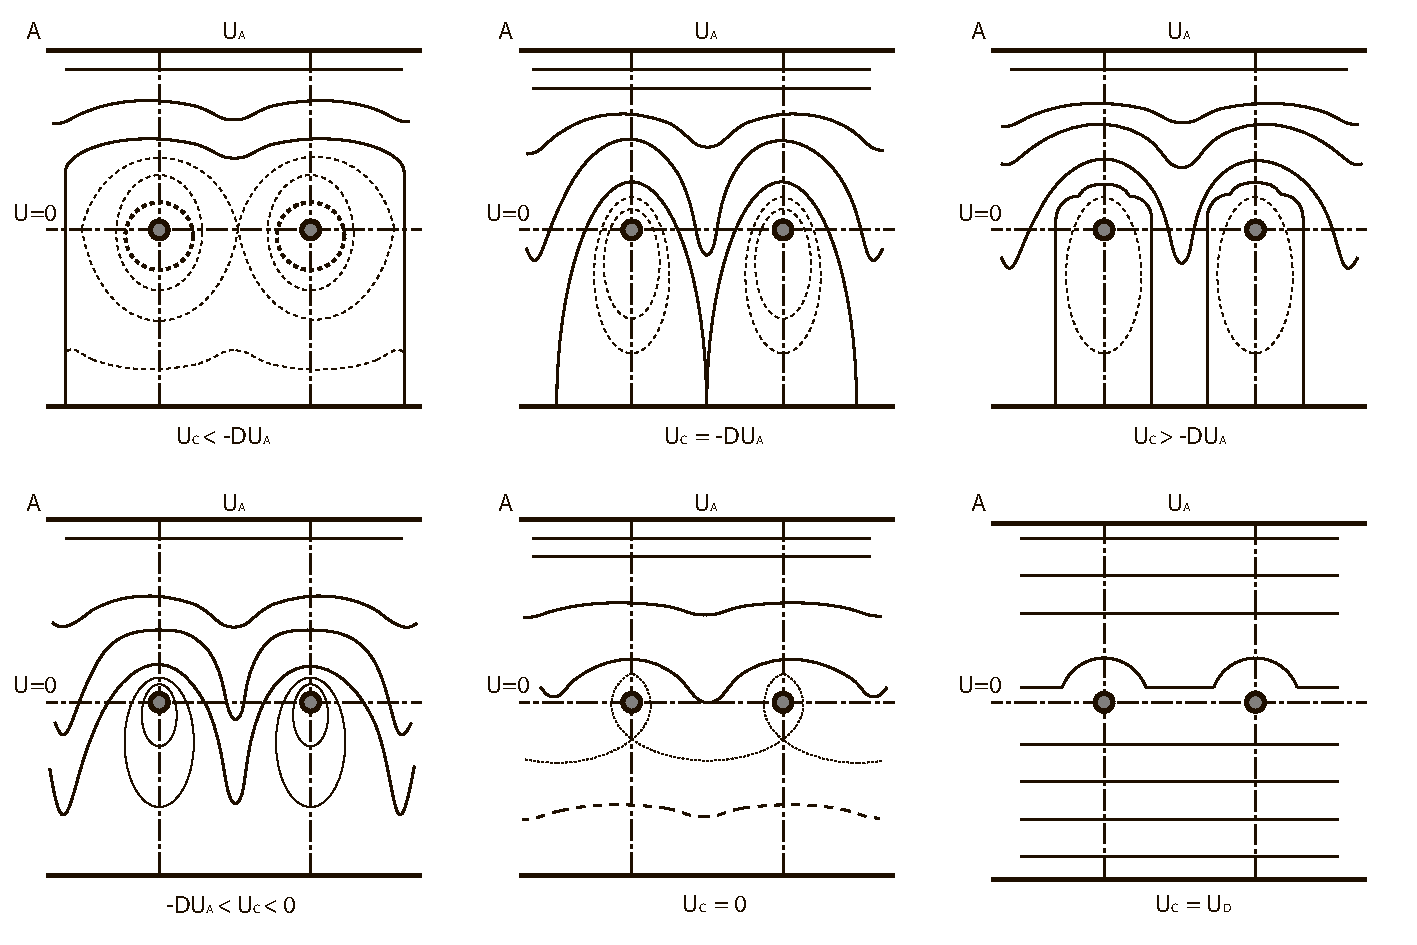
\includegraphics[width=.9\textwidth]{20_U}
  \caption{Распределение электростатического потенциала плоского триода при
  различных потенциалах сетки и одинаковом анодном напряжении}
  \label{pic20U}
\end{figure}
